%---------------------------------- Translatorische Bewegung kombiniert in einem Diagramm für alle Freiheitsgrade--------------------------
\begin{center}
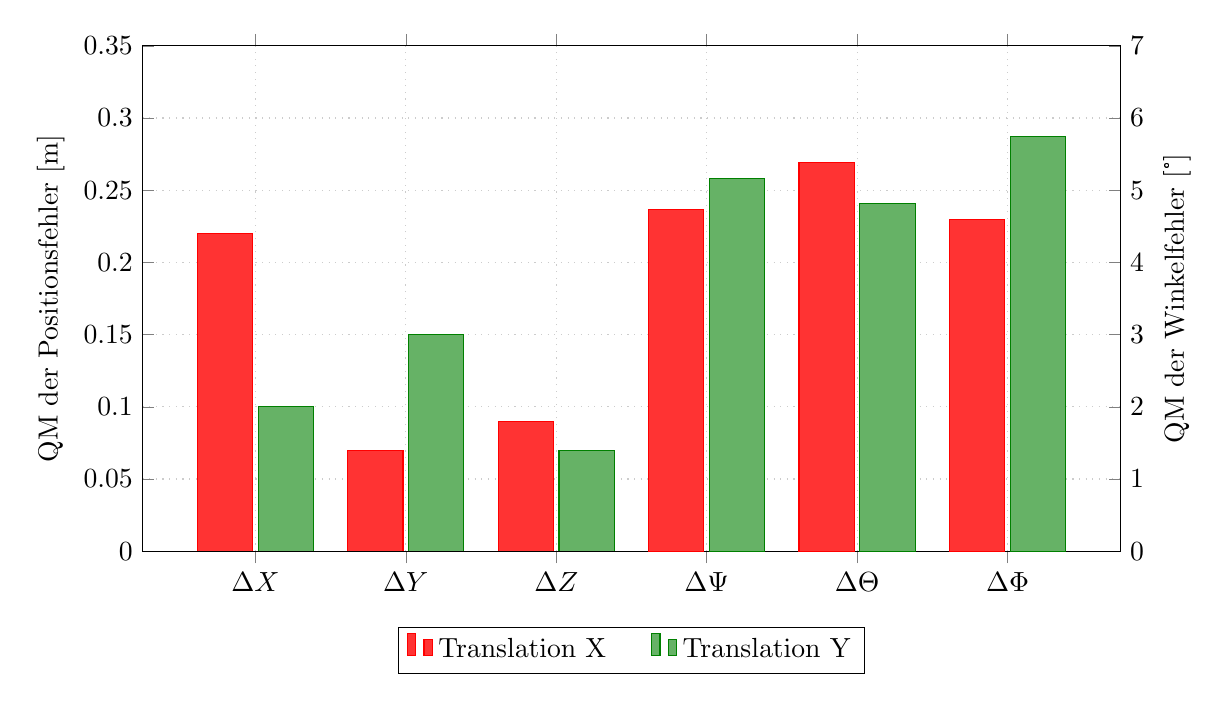
\begin{tikzpicture}
\begin{axis}[
	ybar,
	ymax=0.35,
	ymin=0,
	bar width=20pt,
	scaled y ticks = false,
	y tick label style={/pgf/number format/fixed},
%	enlarge y limits={0.4,upper},
	enlarge x limits=0.15,
	legend style={at={(0.5,-0.15)},
	legend style={/tikz/every even column/.append style={column sep=0.5cm}},
	anchor=north,legend columns=-1},
	ylabel={QM der Positionsfehler \lbrack m\rbrack},
%	symbolic x coords={\Delta,y,z},
	xtick={1,2,3,4,5,6},
	xticklabels={$\Delta X$, $\Delta Y$, $\Delta Z$, $\Delta \Psi$, $\Delta \Theta$, $\Delta \Phi$},
%	xtick=data,
%	every node near coord/.style={/pgf/number format/fixed,/pgf/number format/use comma, anchor=west},
%	nodes near coords,
%	nodes near coords align={vertical},
	width=14cm,
	height=8cm,
	grid=major,
    	grid style={dotted,lightgray!80!white},
    	scaled y ticks = false,
]
\addplot[
%	every node near coord/.append style={xshift=-0.9cm},
%	nodes near coords=\raisebox{0.7cm}{\pgfmathprintnumber\pgfplotspointmeta},
	color=Red,
	fill=Red!80!white,
	bar shift=-11pt,
] coordinates {(1,0.22) (2,0.07) (3,0.09)};
\addplot[
%	every node near coord/.append style={xshift=-0.12cm},
%	nodes near coords=\raisebox{0.7cm}{\pgfmathprintnumber\pgfplotspointmeta},
	color=Green,
	fill=Green!60!white,
	bar shift=11pt,	
] coordinates {(1,0.10) (2,0.15) (3,0.07)};
\addplot[fill opacity=0.0,draw=none,] coordinates {(4,0) (5,0) (6,0)};	%dummy
\legend{Translation X,Translation Y}
\end{axis}

\begin{axis}[
%	scale only axis,
	ybar,
	ymax=7,
	ymin=0,
	bar width=20pt,
%	enlarge y limits={0.4,upper},
	enlarge x limits=0.15,
	legend style={at={(0.5,-0.15)},
	anchor=north,legend columns=-1},
	axis y line*=right,
	ylabel={QM der Winkelfehler \lbrack °\rbrack},
%	symbolic x coords={\Delta,y,z},
	xtick={1,2,3,4,5,6},
	xticklabels={},
%	xtick=data,
%	bar shift=0pt,
%	every node near coord/.style={/pgf/number format/fixed,/pgf/number format/use comma, anchor=west},
%	nodes near coords,
%	nodes near coords align={vertical},
	width=14cm,
	height=8cm,
    	scaled y ticks = false,
]
\addplot[fill opacity=0.0,draw=none,] coordinates {(1,0) (2,0) (3,0)};	%dummy
\addplot[
%	every node near coord/.append style={xshift=-0.9cm},
%	nodes near coords=\raisebox{0.7cm}{\pgfmathprintnumber\pgfplotspointmeta},
	color=Red,
	fill=Red!80!white,
	bar shift=-11pt,	
] coordinates {(4,4.73) (5,5.39) (6,4.59)};
\addplot[
%	every node near coord/.append style={xshift=-0.12cm},
%	nodes near coords=\raisebox{0.7cm}{\pgfmathprintnumber\pgfplotspointmeta},
	color=Green,
	fill=Green!60!white,
	bar shift=11pt,	
] coordinates {(4,5.16) (5,4.82) (6,5.75)};
\end{axis}
\end{tikzpicture}
\end{center}

%----------------------------------------------------------------------------------------------------------
%------------------------------------------  Anfang  ------------------------------------------------------
%------------------------ Vergleich mit xyz rpy in getrennten Diagrammen ----------------------------------
%----------------------------------------------------------------------------------------------------------
%----------------------------------------------------------------------------------------------------------
%\subsection{Translatorische Bewegung}
%\begin{center}
%\begin{tikzpicture}[trim axis left, trim axis right]
%\begin{axis}[
%	ybar,
%	ymax=0.25,
%	ymin=0,
%	bar width=30pt,
%	enlarge x limits=0.4,
%	legend style={at={(0.5,-0.15)},
%	anchor=north,legend columns=-1},
%	ylabel={Positionsfehler \lbrack m\rbrack},
%%	symbolic x coords={\Delta,y,z},
%	xticklabels={$\Delta X$, $\Delta Y$, $\Delta Z$},
%	xtick=data,
%	every node near coord/.style={/pgf/number format/fixed, anchor=west},
%	nodes near coords,
%	nodes near coords align={vertical},
%	width=14cm,
%	height=8cm,
%	grid=major,
%    	grid style={dotted,lightgray!80!white},
%    	scaled y ticks = false,
%	y tick label style={/pgf/number format/fixed},
%]
%\addplot[
%	every node near coord/.append style={xshift=-1.1cm},
%	nodes near coords=\raisebox{0.7cm}{\pgfmathprintnumber\pgfplotspointmeta},
%	color=red,
%	fill=red!30!white
%] coordinates {(-1,0.0942737252) (0,0.0744944439) (1,0.2154737652)};
%\addplot[
%	every node near coord/.append style={xshift=0.0cm},
%	nodes near coords=\raisebox{0.7cm}{\pgfmathprintnumber\pgfplotspointmeta},
%	color=blue,
%	fill=blue!30!white
%] coordinates {(-1,0.0141228693) (0,0.0728502984) (1,0.0578491359)};
%\legend{Translatorsich X,Translatorisch Z}
%\end{axis}
%\label{fig.error_glob_trans}
%\end{tikzpicture}
%\end{center}
%
%\begin{center}
%\begin{tikzpicture}[trim axis left, trim axis right]
%\begin{axis}[
%	ybar,
%	ymax=8,
%	ymin=0,
%	bar width=30pt,
%%	enlarge y limits={0.4,upper},
%	enlarge x limits=0.4,
%	legend style={at={(0.5,-0.15)},
%	anchor=north,legend columns=-1},
%	ylabel={Winkelfehler \lbrack °\rbrack},
%%	symbolic x coords={\Delta,y,z},
%	xticklabels={$\Delta \Psi$, $\Delta \Theta$, $\Delta \Phi$},
%	xtick=data,
%	every node near coord/.style={/pgf/number format/fixed, anchor=west},
%	nodes near coords,
%	nodes near coords align={vertical},
%	width=14cm,
%	height=8cm,
%	grid=major,
%    	grid style={dotted,lightgray!80!white},
%    	scaled y ticks = false,
%	y tick label style={/pgf/number format/fixed},    	
%]
%\addplot[
%	every node near coord/.append style={xshift=-1.1cm},
%	nodes near coords=\raisebox{0.7cm}{\pgfmathprintnumber\pgfplotspointmeta},
%	color=red,
%	fill=red!30!white
%] coordinates {(-1,5.3910094725) (0,0.5944624236) (1,4.7266768476)};
%\addplot[
%	every node near coord/.append style={xshift=0.0cm},
%	nodes near coords=\raisebox{0.7cm}{\pgfmathprintnumber\pgfplotspointmeta},
%	color=blue,
%	fill=blue!30!white
%] coordinates {(-1,3.3292065305) (0,1.4935343647) (1,6.1138224963)};
%\legend{Translatorisch X,Translatorisch Z}
%\end{axis}
%\label{fig.error_loc_trans}
%\end{tikzpicture}
%\end{center}
%----------------------------------------------------------------------------------------------------------
%-------------------------------------------  Ende  -------------------------------------------------------
%------------------------ Vergleich mit xyz rpy in getrennten Diagrammen ----------------------------------
%----------------------------------------------------------------------------------------------------------
%----------------------------------------------------------------------------------------------------------

%----------------------------------------------------------------------------------------------------------
%------------------------------------------  Anfang  ------------------------------------------------------
%---------------- Vergleich mit xyz rpy in einem Diagramm, getrennt nach x und z --------------------------
%----------------------------------------------------------------------------------------------------------
%----------------------------------------------------------------------------------------------------------
%\subsection{Translation X}
%\begin{tikzpicture}
%\begin{axis}[
%	ybar,
%	ymax=0.3,
%	ymin=0,
%	bar width=30pt,
%	scaled y ticks = false,
%	y tick label style={/pgf/number format/fixed},
%% 	enlarge y limits={0.4,upper},
%	enlarge x limits=0.2,
%	legend style={at={(0.5,-0.15)},
%	anchor=north,legend columns=-1},
%	ylabel={Positionsfehler \lbrack m\rbrack},
%% 	symbolic x coords={\Delta,y,z},
%	xtick={1,2,3,4,5,6},
%	xticklabels={$\Delta X$, $\Delta Y$, $\Delta Z$, $\Delta \Psi$, $\Delta \Theta$, $\Delta \Phi$},
%% 	xtick=data,
%	bar shift=0pt,
%	every node near coord/.style={/pgf/number format/fixed, anchor=west},
%	nodes near coords,
%	nodes near coords align={vertical},
%	width=14cm,
%	height=8cm,
%	grid=major,
%	grid style={dotted,lightgray!80!white},
%	scaled y ticks = false,
%]
%\addplot[
%	every node near coord/.append style={xshift=-0.55cm},
%	nodes near coords=\raisebox{0.7cm}{\pgfmathprintnumber\pgfplotspointmeta},
%	color=red,
%	fill=red!30!white
%] coordinates {(1,0.0942737252) (2,0.0744944439) (3,0.2154737652)};
%\addplot[fill opacity=0.0,draw=none,] coordinates {(4,0) (5,0) (6,0)}; %dummy
%%\legend{Raycasting,Endpoint}
%\end{axis}
%
%\begin{axis}[
%% 	scale only axis,
%	ybar,
%	ymax=6,
%	ymin=0,
%	bar width=30pt,
%% 	enlarge y limits={0.4,upper},
%	enlarge x limits=0.2,
%	legend style={at={(0.5,-0.15)},
%	anchor=north,legend columns=-1},
%	axis y line*=right,
%	axis x line=none,
%	ylabel={Winkelfehler \lbrack °\rbrack},
%% 	symbolic x coords={\Delta,y,z},
%	xtick={1,2,3,4,5,6},
%	xticklabels={$\Delta X$, $\Delta Y$, $\Delta Z$, $\Delta \Psi$, $\Delta \Theta$, $\Delta \Phi$},
%% 	xtick=data,
%	bar shift=0pt,
%	every node near coord/.style={/pgf/number format/fixed, anchor=west},
%	nodes near coords,
%	nodes near coords align={vertical},
%	width=14cm,
%	height=8cm,
%	grid=major,
%	grid style={dotted,lightgray!80!white},
%	scaled y ticks = false,
%]
%\addplot[fill opacity=0.0,draw=none,] coordinates {(1,0) (2,0) (3,0)}; %dummy
%\addplot[
%	every node near coord/.append style={xshift=-0.55cm},
%	nodes near coords=\raisebox{0.7cm}{\pgfmathprintnumber\pgfplotspointmeta},
%	color=blue,
%	fill=blue!30!white,
%	% fill opacity=0.5,
%	% draw=none,
%] coordinates {(4,5.3910094725) (5,0.5944624236) (6,4.7266768476)};
%\end{axis}
%\label{fig.error_glob_trans_x}
%\end{tikzpicture}
%
%\subsection{Translation Z}
%\begin{tikzpicture}
%\begin{axis}[
%	ybar,
%	ymax=0.2,
%	ymin=0,
%	bar width=30pt,
%	scaled y ticks = false,
%	y tick label style={/pgf/number format/fixed},
%%	enlarge y limits={0.4,upper},
%	enlarge x limits=0.2,
%	legend style={at={(0.5,-0.15)},
%	anchor=north,legend columns=-1},
%	ylabel={Positionsfehler \lbrack m\rbrack},
%%	symbolic x coords={\Delta,y,z},
%	xtick={1,2,3,4,5,6},
%	xticklabels={$\Delta X$, $\Delta Y$, $\Delta Z$, $\Delta \Psi$, $\Delta \Theta$, $\Delta \Phi$},
%%	xtick=data,
%	bar shift=0pt,
%	every node near coord/.style={/pgf/number format/fixed, anchor=west},
%	nodes near coords,
%	nodes near coords align={vertical},
%	width=14cm,
%	height=8cm,
%	grid=major,
%    	grid style={dotted,lightgray!80!white},
%    	scaled y ticks = false,
%]
%\addplot[
%	every node near coord/.append style={xshift=-0.55cm},
%	nodes near coords=\raisebox{0.7cm}{\pgfmathprintnumber\pgfplotspointmeta},
%	color=red,
%	fill=red!30!white
%] coordinates {(1,0.0141228693) (2,0.0728502984) (3,0.0578491359)};
%\addplot[fill opacity=0.0,draw=none,] coordinates {(4,0) (5,0) (6,0)};	%dummy
%%\legend{Raycasting,Endpoint}
%\end{axis}
%
%\begin{axis}[
%%	scale only axis,
%	ybar,
%	ymax=8,
%	ymin=0,
%	bar width=30pt,
%%	enlarge y limits={0.4,upper},
%	enlarge x limits=0.2,
%	legend style={at={(0.5,-0.15)},
%	anchor=north,legend columns=-1},
%	axis y line*=right,
%	axis x line=none,
%	ylabel={Winkelfehler \lbrack °\rbrack},
%%	symbolic x coords={\Delta,y,z},
%	xtick={1,2,3,4,5,6},
%	xticklabels={$\Delta X$, $\Delta Y$, $\Delta Z$, $\Delta \Psi$, $\Delta \Theta$, $\Delta \Phi$},
%%	xtick=data,
%	bar shift=0pt,
%	every node near coord/.style={/pgf/number format/fixed, anchor=west},
%	nodes near coords,
%	nodes near coords align={vertical},
%	width=14cm,
%	height=8cm,
%	grid=major,
%    	grid style={dotted,lightgray!80!white},
%    	scaled y ticks = false,
%]
%\addplot[fill opacity=0.0,draw=none,] coordinates {(1,0) (2,0) (3,0)};	%dummy
%\addplot[
%	every node near coord/.append style={xshift=-0.55cm},
%	nodes near coords=\raisebox{0.7cm}{\pgfmathprintnumber\pgfplotspointmeta},
%	color=blue,
%	fill=blue!30!white,
%%	fill opacity=0.5,
%%	draw=none,
%] coordinates {(4,3.3292065305) (5,1.4935343647) (6,6.1138224963)};
%%\addplot[
%%	every node near coord/.append style={xshift=-1.1cm},
%%	nodes near coords=\raisebox{0.7cm}{\pgfmathprintnumber\pgfplotspointmeta},
%%	color=red,
%%	fill=red!30!white
%%] coordinates {(-2,0) (-1,0) (0,0) (1,2.4445637073) (2,0.9069805767) (3,8.4545773848)};
%\end{axis}
%\label{fig.error_glob_trans_x}
%\end{tikzpicture}
%----------------------------------------------------------------------------------------------------------
%-------------------------------------------  Ende  -------------------------------------------------------
%--------------------------- Vergleich mit xyz rpy in einem Diagramm --------------------------------------
%----------------------------------------------------------------------------------------------------------
%----------------------------------------------------------------------------------------------------------